

\section{Communication System based on DDM} \label{sec:Communication_Setup_DDM}


The \ac{ddm} method generates transmit signals designed for multiplexing purposes in radar sensing applications. The effects of the transmit signal design due to \ac{ddm} on the communication task are investigated in this section. Based on these investigations, a communication system specifically designed for \ac{ddm} is proposed. In the following, the terms 'receiver' and 'Rx antenna' do not refer to the radar receiver but to the communication receiver.

This section begins with a discussion on different ways to represent the channel for \ac{ddm}, followed by deriving the so-called 'effective' channel. This effective channel is a time-varying \ac{siso} channel that sufficiently describes the communication link between the transmitter and the communication receiver. After that, estimation methods for the effective channel and the transmit data are proposed. 
For these investigations, the waveform and system parameters are chosen according to Tab.~\ref{Tab:com_sys_paramters}. The communication receiver employs only a single Rx antenna, which will turn out to be sufficient for enabling communications. An extension to multiple Rx antennas is straightforward at the cost of additional hardware and an increased power consumption for the communication receiver. 

\begin{table}[!t]
% increase table row spacing, adjust to taste
\renewcommand{\arraystretch}{1.3}
\caption{Waveform and system parameters.}
\label{Tab:com_sys_paramters}
\centering
% Some packages, such as MDW tools, offer better commands for making tables
% than the plain LaTeX2e tabular which is used here.
\begin{tabular}{|l|r|}
\hline
 Parameter & Value  \\
 \hline \hline
 Carrier frequency $f_\text{c}$ & $77 \, \text{GHz}$ \\
 \hline
 Bandwidth $B$ & $1\, \text{GHz}$ \\
 \hline
 Number of subcarriers $N_\text{c}$ & $1024$ \\
 \hline
 \ac{adc} sampling time $T_\text{s}$  &  $1\, \text{ns}$ \\
 \hline
 Subcarrier spacing $\Delta f$ & $976.5 \, \text{MHz}$ \\
 \hline
 
 Length of an OFDM symbol $T$ & $1.024\,$\textmu$\text{s}$ \\
 \hline
 Length of the cyclic prefix $T_\text{cp}$ & $1\,$\textmu$\text{s}$ \\
 \hline
 Number of \ac{ofdm} symbols $N_\text{sym}$ & $512$ \\
 \hline
  Number of Rx antennas $N_\text{Rx}$ & $1$ \\
 \hline
 Number of Tx antennas $N_\text{Tx}$ & $4$ \\
 \hline
  Symbol alphabet & QPSK \\
 \hline
 Phase shift $\Delta \psi_k$ &  $\{ -\frac{3 \pi}{4}, -\frac{1 \pi}{4}, \frac{1 \pi}{4}, \frac{3 \pi}{4}\}$ \\
 \hline
\end{tabular}
\end{table}


\subsection{Channel Model} 



%\newcommand\DELTA{0.5}
\begin{figure*}[!t]
\centering
\begin{tikzpicture}[scale=0.8, style=thick, rounded corners=1pt,inner sep=3.2pt,node distance=.8cm,every text node part/.style={align=center}]
%\tikzset{
%    mynode/.style={sharp corners=2pt,inner sep=7pt,node distance=.8cm,every text node part/.style={align=center}},
%    myarrow/.style={->, >=latex', shorten >=1pt, thick},
%    mylabel/.style={text width=7em, text centered} ,
%    classical/.style={thick,->,>=stealth},
%    cirarrow/.style={thick,->,>=stealth, dashed,shorten >=4pt,shorten <=4pt},
%}

% Draw rectangular nodes (switch sharp to smooth for different corners)
\node[ minimum height = 1cm, minimum width = 1cm] (state0){\small Transmit data \\ $\m{S} \in \mathbb{C}^{N_\text{c} \times N_\text{sym}}$};

\node[above right =-0.8cm and 1.8cm of state0, minimum height = 0cm, minimum width = 0cm]{ $\vdots $};
\node[above right =-0.8cm and 3.9cm of state0, minimum height = 0cm, minimum width = 0cm]{ $\vdots $};
\node[above right =-0.8cm and 5.6cm of state0, minimum height = 0cm, minimum width = 0cm]{ $\vdots $};

\node[draw, above right =-0.2cm and 1cm of state0, minimum height = 1cm, minimum width = 1cm](state1u){\small $ \cdot\m{D}_{N_\text{sym}} \left( \frac{\Delta \psi_0}{2 \pi} \right)  $};

\node[draw, below right =-0.2cm and 1cm of state0, minimum height = 1cm, minimum width = 1cm](state1d){\small $ \cdot \m{D}_{N_\text{sym}} \left( \frac{\Delta \psi_3}{2 \pi} \right)  $};

\draw[->] (state0.east)  -- ++(0.5cm,0) -- ++(0,1.035cm) -- (state1u.west);
\draw[->] (state0.east)  -- ++(0.5cm,0) -- ++(0,-1.035cm) -- (state1d.west);

\node[draw,right=0.5cm of state1u, minimum height = 1cm, minimum width = 1cm](state2u){\small $\m{F}_{N_\text{c}}^{-1} \downarrow$};
\node[draw,right=0.5cm of state1d, minimum height = 1cm, minimum width = 1cm](state2d){\small $\m{F}_{N_\text{c}}^{-1} \downarrow$};

\draw[->] (state1u.east)  -- (state2u.west);
\draw[->] (state1d.east)  -- (state2d.west);

\node[draw,right=0.5cm of state2u, minimum height = 1cm, minimum width = 1cm](state3u){\small Add CP};
\node[draw,right=0.5cm of state2d, minimum height = 1cm, minimum width = 1cm](state3d){\small Add CP};

\draw[->] (state2u.east)  -- (state3u.west);
\draw[->] (state2d.east)  -- (state3d.west);

%\node[draw,right=0.5cm of state3u, minimum height = 1cm, minimum width = 1cm](state4u){\small Analog \\ front-end};
%\node[draw,right=0.5cm of state3d, minimum height = 1cm, minimum width = 1cm](state4d){\small Analog \\ front-end};
%
%\draw[->] (state3u.east)  -- (state4u.west);
%\draw[->] (state3d.east)  -- (state4d.west);

\draw (state3u.east)  -- ++(0.5,0) coordinate (Ant1u);
\draw (Ant1u)  -- ++(0,0.4) coordinate (IntAnt1u);
\draw (IntAnt1u)  -- ++(-0.2,0.3);
\draw (IntAnt1u)  -- ++(0.2,0.3);

\draw (state3d.east)  -- ++(0.5,0) coordinate (Ant1d);
\draw (Ant1d)  -- ++(0,0.4) coordinate (IntAnt1d);
\draw (IntAnt1d)  -- ++(-0.2,0.3);
\draw (IntAnt1d)  -- ++(0.2,0.3);


%\node[draw,below right =0cm and 2cm of state3u, minimum height = 1cm, minimum width = 1cm](state5){\small Analog \\ front-end};

\node[draw,below right =-0.2cm and 2cm of state3u, minimum height = 1cm, minimum width = 1cm](state6){\small Remove \\ CP};

\draw (state6.west)  -- ++(-0.5,0) coordinate (Ant2);
\draw (Ant2)  -- ++(0,0.4) coordinate (IntAnt2);
\draw (IntAnt2)  -- ++(-0.2,0.3);
\draw (IntAnt2)  -- ++(0.2,0.3);

\draw [->, shorten <=0.2cm, shorten >=0.2cm, style=dashed] (IntAnt1u) to [out=-20,in=160] (IntAnt2);
\draw [->, shorten <=0.2cm, shorten >=0.2cm, style=dashed] (IntAnt1d) to [out=20,in=200] (IntAnt2);



%\draw[->] (state5.east)  -- (state6.west);

\node[draw,right=0.5cm of state6, minimum height = 1cm, minimum width = 1cm](state7){\small $\m{F}_{N_\text{c}} \downarrow$};

\draw[->] (state6.east)  -- (state7.west);

\node[right=0.5cm of state7, minimum height = 0cm, minimum width = 0cm](state8){};

\draw[->] (state7.east)  -- (state8.west);


\node[below right =0.05cm and 0.0cm of state3d.east, minimum height = 0cm, minimum width = 0cm](cb1){};

\draw [decorate,decoration={brace,mirror, amplitude=8pt},xshift=0pt,yshift=0pt]
(cb1) -- ++(2.1,0.0) node [black,midway,yshift=-0.45cm] 
{\footnotesize CIR $\ve{f}_k$};


\node[below right =0.65cm and 0.0cm of state1d.east, minimum height = 0cm, minimum width = 0cm](cb1){};

\draw [decorate,decoration={brace,mirror, amplitude=8pt},xshift=0pt,yshift=0pt]
(cb1) -- ++(10.5,0.0) node [black,midway,yshift=-0.45cm] 
{\footnotesize CFR $\ve{p}_k$};


\node[below right =2.10cm and -0.2cm of state0.east, minimum height = 0cm, minimum width = 0cm](cb1){};

\draw [decorate,decoration={brace,mirror, amplitude=8pt},xshift=0pt,yshift=0pt]
(cb1) -- ++(14.5,0.0) node [black,midway,yshift=-0.45cm] 
{\footnotesize ECFR  $\m{H}$};


%
%\draw[cirarrow] (IntAnt1) -- (RxIntAnt1);
%\draw[cirarrow] (IntAnt2) -- (RxIntAnt1);
%
%\draw[draw=black, style=dashed, fill=none] (3.7,-1.6) rectangle ++(2.6, 3.9);
%\node at (5.2,-1.35) {\small CIRs/CFRs};
%
%\draw[draw=black, style=dashed, fill=none] (0.1,-2.4) rectangle ++(6.25, 4.8);
%\node at (5.2,-2.2) {\small ECIR/ECFR};
%
%\node[below of = IntAnt1, node distance=1.1cm] {$\vdots$}; 

\end{tikzpicture}
\caption{Transmitter and receiver processing chains including the CIR, the CFR, and the ECFR with their covered processing blocks. The parallel-to-serial conversions, the DACs, the ADC, and the analog front-ends are not shown for simplicity. The figure is based on a similar figure in \cite{Lang_RDM_JP}.}
\label{fig:Comm_setup_ECIR}
\end{figure*}





Fig.~\ref{fig:Comm_setup_ECIR} shows the processing blocks for \ac{ddm} in the transmitter, the $N_\text{Tx}$ \acp{cir} from each Tx antenna to the Rx antenna, and the first two receiver processing blocks. On basis of that, we will introduce different channel representations


%The basic transmitter signal processing chain for \ac{ddm}, the $N_\text{Tx}$ \acp{cir} from each Tx antenna to the Rx antenna, and the first two receiver processing blocks are visualized in Fig.~\ref{fig:Comm_setup_ECIR}. For every antenna index $k$, the transmitter applies the phase shift via $\m{D}_{N_\text{sym}} \left( \frac{\Delta \psi_k}{2 \pi} \right)$ on matrix $\m{S}$ containing the subcarrier symbols. The result is transformed into time domain, extended by a \ac{cp}, and convolved with the $N_\text{Tx}$ individual \acp{cir}. The receiver removes the \ac{cp} and transforms the received \ac{ofdm} symbols into frequency domain. 

As for \ac{rdm} in \cite{Lang_RDM_JP}, the channel for \ac{ddm} can be represented in three possible ways. 

\subsubsection{CIR Representation} 

A straightforward way of describing the channel is to utilize the $N_\text{Tx}$ individual \acp{cir}. The model for these \acp{cir} \cite{Rappaport_SISO_Channel, Rappaport_SISO_Channel_JP, Code_MIMO_Channels} and the model parametrization are equal to that employed in \cite{Lang_RDM_JP}, such that a detailed description is omitted in this work. These \acp{cir} are denoted as $\ve{f}_k \in \mathbb{C}^{N_\ve{f}}$ for $0 \leq k < N_\text{Tx}$ and their assumed length is $N_\ve{f} = 256$. 

\subsubsection{CFR Representation} 

Another way is to utilize the \acp{cfr}, which describe the $N_\text{Tx}$ individual \acp{cir} in frequency domain. 
%Each \ac{cfr} contains $N_\text{Tx}$ individual \acp{cir} as well as several processing steps in the transmitter and receiver. 
These \acp{cfr} are denoted as  $\ve{p}_k \in \mathbb{C}^{N_\text{c}}$ and are given by
\begin{align}
 \ve{p}_k = \m{F}_{N_\text{c}} \m{B}_{\text{zp}} \ve{f}_k, \label{equ:Comm_OFDM_ECIR_002o}
\end{align}
where the matrix $\m{B}_{\text{zp}}\in \mathbb{C}^{N_\text{c} \times N_\ve{f}}$ zero-pads the \acp{cir} $\ve{f}_k$ to a length of $N_\text{c}$. 


\subsubsection{ECFR Representation} 

Here, we exploit the fact that all antennas transmit the same subcarrier symbols $\m{S}$ up to the deterministic phase shift $\Delta \psi_k$. Thus, the third way of describing the channel covers all shown processing blocks in Fig.~\ref{fig:Comm_setup_ECIR}. This channel representation is referred to as \ac{ecfr}, which can be modeled as a \ac{siso} channel despite the fact that several Tx antennas are involved. 

The \ac{ecfr} is mathematically described in the following. 
%This mathematical description is based on the assumption that the \acp{cir} and the \acp{cfr} are static. A potential time-dependency due to a relative velocity between transmitter and receiver is discussed later.
As depicted in Fig.~\ref{fig:Comm_setup_ECIR}, the \ac{ecfr} covers the \acp{cfr} and the diagonal matrices $\m{D}_{N_\text{sym}} \left( \frac{\Delta \psi_k}{2 \pi} \right)$. These diagonal matrices apply a phase shift from \ac{ofdm} symbol to \ac{ofdm} symbol. Thus, the \ac{ecfr} will change from \ac{ofdm} symbol to \ac{ofdm} symbol. Let $ \m{H} \in \mathbb{C}^{N_\text{c} \times N_\text{sym}}$ denote the \ac{ecfr} for all $N_\text{sym}$ \ac{ofdm} symbols, then, $ \m{H}$ is given by
\begin{align}
 \m{H} = \sum_{k=0}^{N_\text{Tx}-1} \m{Q}_k, \label{equ:Comm_OFDM_ECIR_002}
\end{align}
where the matrices $\m{Q}_k \in \mathbb{C}^{N_\text{c} \times N_\text{sym}}$ are given as
\begin{align}
 \m{Q}_k &={}  \ve{p}_k \left( \ve{1}^{N_\text{sym}} \right)^T \m{D}_{N_\text{sym}} \left( \frac{\Delta \psi_k}{2 \pi} \right) \\
 &={}  \ve{p}_k  \ve{d}_{N_\text{sym}} \left( \frac{\Delta \psi_k}{2 \pi} \right)^T. \label{equ:Comm_OFDM_ECIR_002qw}
\end{align}
Each matrix $\m{Q}_k$ for $0 \leq k < N_\text{Tx}$ represents one signal path in Fig.~\ref{fig:Comm_setup_ECIR}.

%This \ac{ecfr} turns out to be heavily time-varying, which is discussed in the following.
    
\subsubsection{Properties of the ECFR} \label{sec:Discussion_ECFR}
    
Note that the $N_\text{Tx}$ different terms used to construct the \ac{ecfr} in \eqref{equ:Comm_OFDM_ECIR_002} may interfere constructively or destructively. On top of that, this constructive/destructive interference turns out to be heavily time-varying. 

The time-dependency of the \ac{ecfr} can be well demonstrated for \ac{awgn} channels where  $\m{Q}_k$ in \eqref{equ:Comm_OFDM_ECIR_002qw} reduces to 
\begin{align}
 \m{Q}_k =  \ve{1}^{N_\text{c}} \ve{d}_{N_\text{sym}} \left( \frac{\Delta \psi_k}{2 \pi} \right)^T.   \label{equ:Comm_OFDM_ECIR_002ay}
\end{align}
According to \eqref{equ:Comm_OFDM_ECIR_002ay}, all subcarriers experience the same effects. It is thus sufficient to inspect a single subcarrier, e.g, the first one. 

This subcarrier is represented by the first row of $\m{Q}_k$ denoted as $\left[\m{Q}_k \right]_{0,\mu}$, where the \ac{ofdm} symbols are indexed with $0 \leq \mu < N_\text{sym}$. The magnitude and phase values for these elements are exemplarily sketched in form of arrows in the complex plane in Tab.~\ref{table_phase_rotations} for the first 9 \ac{ofdm} symbols $0 \leq \mu < 9$ and for the choice of $\Delta \psi_k = \{ \frac{1 \pi}{4}, \frac{3 \pi}{4}, \frac{5 \pi}{4}, \frac{7 \pi}{4}\}$. According to \eqref{equ:Comm_OFDM_ECIR_002}, the sum of the elements $\left[\m{Q}_k \right]_{0,\mu}$ for $0 \leq k < N_\text{Tx}$ yields the first subcarrier of the \ac{ecfr} $\left[\m{H} \right]_{0,\mu}$ for the $\mu$th \ac{ofdm} symbol, which is also sketched in Tab.~\ref{table_phase_rotations}. 
One can see, that for $\mu = 0$ all components add up constructively. Hence, the \ac{ecfr} can be considered to be good and the received signal power will be maximized for this \ac{ofdm} symbol. The next three \ac{ofdm} symbols observe destructive interference leading to full cancellation of the signal components, such that the received signal power is zero. For the \ac{ofdm} symbols $\mu=4, \hdots 7$ the arrows point in the opposite direction than for $\mu=0, \hdots 3$, respectively. This pattern repeats for $\mu \geq 8$. 
%Thus, it holds that $\left[\m{Q}_k \right]_{0,\mu} = -\left[\m{Q}_k \right]_{0,\mu+4}$ as well as $\left[\m{H} \right]_{1,\mu} =- \left[\m{H} \right]_{1,\mu+4}$ for $\mu=0, \hdots 3$. At $\mu=8$, we observe the same arrows as for $\mu=0$, indicating a periodically occurrence of the constructive/destructive interference. 
For the \ac{awgn} case, we notice that constructive/destructive interference is observed with a period of 8 \ac{ofdm} symbols. Within this period, the \ac{ecfr} for the first 4 \ac{ofdm} symbols equals that for the subsequent 4 \ac{ofdm} symbols when inverting all signs. 




\begin{table}[!t]
% increase table row spacing, adjust to taste
\renewcommand{\arraystretch}{1.20}
\caption{Schematic visualization of the elements of $\left[\m{Q}_k \right]_{0,\mu}$ for $0 \leq k < N_\text{Tx}$ and for $0 \leq \mu < 9$ in case of \ac{awgn} channels.}
\label{table_phase_rotations}
\centering
% Some packages, such as MDW tools, offer better commands for making tables
% than the plain LaTeX2e tabular which is used here.
\begin{tabular}{|c|c|c|c|c|c|c|c|c|c|}
\hline
 $\mu$&  0 & 1 & 2 & 3 & 4 & 5 & 6 & 7 & 8 \\
 \hline \hline
 $\left[\m{Q}_0 \right]_{0,\mu}$ &  $\rightarrow$ &  $\myswarrow$ &  $\uparrow$ &  $\mysearrow$ &  $\leftarrow$ & $\mynearrow$ & $\downarrow$ &  $\mynwarrow$ &  $\rightarrow$ \\
 \hline
  $\left[\m{Q}_1 \right]_{0,\mu}$ &  $\rightarrow$ &  $\mysearrow$ &  $\downarrow$ &  $\myswarrow$ &  $\leftarrow$ & $\mynwarrow$ & $\uparrow$ & $\mynearrow$ &  $\rightarrow$ \\
 \hline
  $\left[\m{Q}_2 \right]_{0,\mu}$ &   $\rightarrow$ &  $\mynearrow$ &  $\uparrow$ &  $\mynwarrow$ &  $\leftarrow$ & $\myswarrow$ & $\downarrow$ & $\mysearrow$ &  $\rightarrow$ \\
 \hline
  $\left[\m{Q}_3 \right]_{0,\mu}$ &  $\rightarrow$ &  $\mynwarrow$ &  $\downarrow$ &  $\mynearrow$ &  $\leftarrow$ & $\mysearrow$ & $\uparrow$ &  $\myswarrow$ &  $\rightarrow$ \\
 \hline \hline
 $\left[\m{H} \right]_{0,\mu}$ &  $\Largerightarrow$ &  0 &  0 &  0 &  $\Largeleftarrow$ & 0 & 0 &  0 &  $\Largerightarrow$ \\
 \hline
\end{tabular}
\end{table}



The same analysis for the employed frequency selective channel model \cite{Lang_RDM_JP} is presented in the following. For this model, the magnitude values of $\left[\m{H} \right]_{0,\mu}$ for an exemplary \ac{ecfr} are shown in Fig.~\ref{fig:MIMO_channel_pattern}.  Since the real-valued magnitude rather than the complex-valued amplitude values are shown, a period of 4 \ac{ofdm} symbols is observed. Within these 4 \ac{ofdm} symbols one can observe a pattern where 3 \ac{ofdm} symbols experience a rather strong attenuation, making a successful transmission difficult. Consequently, robustifying the communication is necessary.





\begin{figure}[!t]
\begin{center}
\begin{tikzpicture}
\begin{axis}[compat=newest, 
width=0.8\columnwidth, height = .5\columnwidth, xlabel={OFDM symbol index $\mu$}, 
ylabel style={align=center}, 
ylabel style={text width=3.4cm},
ylabel={Normalized power of $\left[\m{H} \right]_{0,\mu}$ (dB)}, 
legend pos=north east, 
legend cell align=left,
legend columns=2, 
        legend style={
                    % the /tikz/ prefix is necessary here...
                    % otherwise, it might end-up with `/pgfplots/column 2`
                    % which is not what we want. compare pgfmanual.pdf
            /tikz/column 2/.style={
                column sep=5pt,
            },
        font=\small},
xmin = 0,
xmax = 15,
ymax = 0,
ymin = -25,
grid=major,
%restrict y to domain=-inf:20,
legend style={
at={(-0.25,1.6)},
anchor=north west}
]

% H abs norm 
\addplot[line width=1pt, color=black, style=solid] table[x index =0, y index =2] {fig/MIMO_channel_pattern_DDM.dat};
%\addlegendentry{{LS est.}}
\label{p1}

%% LOS max
%\addplot[line width=1pt, color=black, style=dashed] table[x index =0, y index =2] {fig/SISO_channel_stats.dat};
%%\addlegendentry{{WLLS est.}}
%\label{p2}

%% NLOS avg 
%\addplot[line width=1pt, color=gray, style=solid] table[x index =0, y index =3] {fig/SISO_channel_stats.dat};
%%\addlegendentry{{Real part of the LS est.}}
%\label{p3}

%% NLOS max
%\addplot[line width=1pt, color=gray, style=dashed] table[x index =0, y index =4] {fig/SISO_channel_stats.dat};
%%\addlegendentry{{BWLUE}}
%\label{p4}

         
\end{axis}
%\node [draw,fill=white,anchor=north east] at (rel axis cs: 0.98,0.98) {\shortstack[l]{
%	\begin{tabular}{l}
%		\ref{p1} \small LOS  \\
%  		\ref{p3} \small NLOS 
%\end{tabular}}} ;



\end{tikzpicture}
\caption{Normalized power of the first subcarrier of an exemplary frequency selective ECFR plotted over the OFDM symbol index $\mu$.  \label{fig:MIMO_channel_pattern} }
\end{center}
\end{figure}





\subsubsection{Increasing Robustness of the Communication}
\label{sec:Robust_DDM}

In wireless communications, bad channel conditions are usually tackled by adding redundancy to the transmit data. As discussed in \cite{Lang_RDM_JP}, redundancy may be added using an adequate channel code. Here, we face the same problem as in \cite{Lang_RDM_JP} for \ac{rdm}, where a usually sufficing convolutional code with code rate $r=1/2$ was not powerful enough to overcome the interference pattern in the \acp{ecfr}. 
%Using a channel code with a lower code rate would probably be able to handle these distortions, but also significantly increase the computational complexity of the corresponding channel decoder, and thus, limit its applicability. 

%Another fact worth being considered is that the channel decoder in general does not work well for burst errors. This is in contrast to the observed pattern in Fig.~\ref{fig:MIMO_channel_pattern}, which indicates that burst errors may occur frequently.

The approach proposed in this work is similar to the one used in \cite{Lang_RDM_JP}. We propose adding redundancy to the transmit data by sending the same subcarrier symbols on $4$ consecutive \ac{ofdm} symbols in combination with a channel code with a code rate of $r=1/2$. The former one can be implemented with very low complexity and is inspired by space-time codes \cite{lu2000space, alamouti1998simple, tarokh1998space}, which utilize diversity gain to robustify  the transmission in difficult environments. The proposed approach also utilizes diversity gain, which will result in an increased \ac{ber} performance as will be shown later in this work. 

As discussed in \cite{Lang_RDM_JP}, adding redundancy  reduces the data rate, which may be seen as a moderate disadvantage for automotive \ac{ofdm} joint radar and communication systems, since the large bandwidths employed allow for very high data rates that exceed those of competitive radar waveforms significantly \cite{8897604}. 


Transmitting the same subcarrier symbols on $4$ consecutive  \ac{ofdm} symbols is mathematically described by constructing  $\m{S}$ according to
\begin{align}
\m{S} =  \m{X} \m{B},  \label{equ:Comm_OFDM_00111}
\end{align}
with $\m{B}$ given as
\begin{align}
\m{B} &={} \left[ \begin{smallmatrix}
&  &  &  \\
1 & 1 & 1 & 1   & 0 & 0 & 0 & 0   & 0 & 0 & 0 & 0   & 0 & 0 & 0 & 0   &   \\
0 & 0 & 0 & 0   & 1 & 1 & 1 & 1   & 0 & 0 & 0 & 0   & 0 & 0 & 0 & 0   & \hdots \\
0 & 0 & 0 & 0   & 0 & 0 & 0 & 0   & 1 & 1 & 1 & 1   & 0 & 0 & 0 & 0   &  \\
0 & 0 & 0 & 0   & 0 & 0 & 0 & 0   & 0 & 0 & 0 & 0   & 1 & 1 & 1 & 1   &  \\
  & & \vdots & &   & &  \vdots & &   & & \vdots  &  &  & & \vdots  & & \ddots \\
\end{smallmatrix} \right]  \in \mathbb{R}^{(N_\text{sym}/4) \times N_\text{sym}}. \label{equ:IEEE_DDM_Bperm} 
\end{align} 
%This way, the subcarrier symbols in every column in $\m{X}\in \mathbb{C}^{N_\text{c} \times N_\text{sym}/4}$ are spread over 4 consecutive \ac{ofdm} symbols in $\m{S}$. 


\subsection{Signal Model} 

%It turns out using a notation that fits to the introduced redundancy within $\m{S}$ makes the following mathematical expressions simpler. 
For the mathematical description, $4$ consecutive \ac{ofdm} symbols within $\m{S}$ carrying the same subcarrier symbols are referred to as a bundle. Hence, $\m{S}$ contains $N_\text{sym}/4$ bundles indexed with $0 \leq \kappa < N_\text{sym}/4$. Within every bundle, the 4 \ac{ofdm} symbols are indexed with $0 \leq \gamma < 4$. This notation is visualized in Fig.~\ref{fig:Comm_setup_DDM}, which sketches the rows and columns of $\m{S}$. The columns of $\m{S}$ are denoted as $\ve{s}_{\kappa, \gamma} \in \mathbb{C}^{N_\text{c}}$ with $\kappa$ and $\gamma$ indicating the corresponding bundle and the \ac{ofdm} symbol within this bundle, respectively. The columns of the matrix $\m{X}$ are denoted as $\ve{x}_{\kappa} \in \mathbb{C}^{N_\text{c}}$.  This way, it holds that $\ve{x}_{\kappa} = \ve{s}_{\kappa, \gamma} $ for $0 \leq \gamma < 4$. 
 
Next, a mathematical model of the received time domain \ac{ofdm} symbols is derived. This model is similar to \eqref{equ:MIMO_OFDM_011} except that it applies to the communication receiver rather than the radar receiver. Hence, it uses the \ac{ecfr} discussed for the communication task. With $\m{P}_k = \text{diag}\left( \ve{p}_k \right)$, \eqref{equ:MIMO_OFDM_010}, \eqref{equ:Comm_OFDM_ECIR_002}, \eqref{equ:Comm_OFDM_ECIR_002qw}, and  \eqref{equ:Comm_OFDM_00111}, this model is given by
\begin{align}
	\m{Y}_{\text{tf,ts}} &={} \sum_{k=0}^{N_\text{Tx}-1} \m{F}_{N_\text{c}}^{-1} \m{P}_k \m{S}_k  \m{\Lambda} + \m{N} \label{equ:ECFR1_OFDM_011} \\
	&={} \sum_{k=0}^{N_\text{Tx}-1} \m{F}_{N_\text{c}}^{-1} \m{P}_k \m{S}  \m{D}_{N_\text{sym}} \left( \frac{\Delta \psi_k}{2 \pi} \right) \m{\Lambda}  + \m{N} \\
	 &={}  \m{F}_{N_\text{c}}^{-1} \left( \m{H} \odot \m{S} \right) \m{\Lambda} + \m{N}\\
	 &={}  \m{F}_{N_\text{c}}^{-1} \left( \m{H} \odot \left( \m{X} \m{B} \right) \right) \m{\Lambda} + \m{N}.\label{equ:ECFR2_OFDM_011}
\end{align}
Similar to \cite{Lang_RDM_JP}, the diagonal matrix $\m{\Lambda} \in \mathbb{C}^{N_\text{sym} \times N_\text{sym}}$ models the \acp{cpe}. Its diagonal elements are given by $\text{e}^{\text{j} \varphi_{\kappa, \gamma}}$ with $ \varphi_{\kappa, \gamma}$ representing the unknown \ac{cpe} for the $\gamma$th \ac{ofdm} symbol within the $\kappa$th bundle. The matrix $\m{N} \in \mathbb{C}^{N_\text{c} \times N_\text{sym}}$ represents zero-mean white Gaussian measurement noise, whose uncorrelated elements have a variance of $\sigma_\text{n}^2$.
% $[N]_{k,l} \sim \mathcal{N}(0,\sigma_\text{n}^2)$


Recall that the \ac{ecfr} $\m{H}$ shows a period of 8 columns. Within this period, the columns of $\m{H}$ show a pattern where the first 4 columns are equal with the following 4 columns when inverting all signs. This pattern is accounted for by inverting the signs of the received signals for the corresponding \ac{ofdm} symbols as described in the following. 
Let $\ve{y}_{\kappa, \gamma} \in \mathbb{C}^{N_\text{c}}$ be the column of $\m{Y}_{\text{tf,ts}}$ corresponding to the $\gamma$th \ac{ofdm} symbol within the $\kappa$th bundle, and let $\ve{z}_{\kappa, \gamma} \in \mathbb{C}^{N_\text{c}}$ be its \ac{dft} transform up to a sign inversion in case of odd vales of $\kappa$
\begin{align}
	\ve{z}_{\kappa, \gamma} &={} \left(-1\right)^{\kappa} \m{F}_{N_\text{c}} \ve{y}_{\kappa, \gamma}. \label{equ:IEEE_CIR032kappa} 
\end{align}
The follow-up receiver signal processing is based on $\ve{z}_{\kappa, \gamma}$ rather than on $\ve{y}_{\kappa, \gamma}$, which allows describing the \ac{ecfr} $\m{H}$ by only 4 columns. These 4 columns will be denoted as $\ve{h}_{\gamma} \in \mathbb{C}^{N_\text{c}}$ for $\gamma = 0, \hdots, 3$. From now on, these 4 vectors are referred to \ac{ecfr} for the sake of simplicity. A diagonal matrix with the \ac{ecfr} is defined as $\m{H}_{\gamma} = \text{diag}\left( \ve{h}_{\gamma}  \right)\in \mathbb{C}^{N_\text{c} \times N_\text{c}}$.

The \ac{ecfr} $\ve{h}_{\gamma}$ transformed into the time domain is denoted as \ac{ecir} $\ve{g}_{\gamma}\in \mathbb{C}^{N_\ve{g}}$, whose length $N_\ve{g}$ corresponds to the length of the \ac{cir} $\ve{f}_{k}$ of  $N_\ve{f} = N_\ve{g} = 256$. The \ac{ecir} and the \ac{ecfr} are connected via
\begin{align}
\ve{h}_{\gamma} = \m{F}_{N_\text{c}} \m{B}_{\text{zp}} \ve{g}_{\gamma}. \label{equ:DDM_001}
\end{align}
The introduced definitions and notations allow simplifying the model in \eqref{equ:ECFR1_OFDM_011}--\eqref{equ:ECFR2_OFDM_011} as
\begin{align}
	\ve{z}_{\kappa, \gamma} &={} \m{H}_{\gamma} \ve{s}_{\kappa, \gamma} \text{e}^{\text{j} \varphi_{\kappa, \gamma}} + \ve{n}_{\kappa, \gamma} \label{equ:MODEL_DDM_prea001} \\
	&={} \m{H}_{\gamma}  \ve{x}_{\kappa} \text{e}^{\text{j} \varphi_{\kappa, \gamma}} + \ve{n}_{\kappa, \gamma} , \label{equ:MODEL_DDM_prea002} 
\end{align}
where $\ve{n}_{\kappa,\gamma}\in \mathbb{C}^{N_\text{c}}$ is a white Gaussian noise vector given by the \ac{dft} of the corresponding columns of $\m{N}$. The alternating sign considered in \eqref{equ:IEEE_CIR032kappa} is ignored for the noise, since it does not affect its statistics. The covariance matrix of $\ve{n}_{\kappa,\gamma}$ is given by $\m{C}_{\ve{n}\ve{n}}=N_\text{c} \sigma_\text{n}^2 \m{I}^{N_\text{c}}$. 

The matrix $\m{S}$ contains $N_\text{pr}$ preamble \ac{ofdm} symbols in the first $N_\text{pr}$ columns, which are used for channel estimation later in this work. Thus, $\m{X}$ contains $N_\text{pr}/4$ preamble \ac{ofdm} symbols in the first $N_\text{pr}/4$ columns, where it is assumed that $N_\text{pr}$ is a multiple of 4. Let $\ve{x}_\text{pr}\in \mathbb{C}^{N_\text{c}}$ be the preamble \ac{ofdm} symbol in frequency domain such that $\ve{x}_{\kappa} = \ve{x}_\text{pr}$ for $0 \leq \kappa < N_\text{pr}/4$. 
%An exemplary allocation of 4 preamble \ac{ofdm} symbols is sketched in Fig.~\ref{fig:Comm_setup_DDM}.

For $\kappa \geq N_\text{pr}/4$, $\ve{x}_{\kappa}$ consists of $N_\text{p}$ pilot and $N_\text{d}$ data subcarriers such that $N_\text{c} = N_\text{p} + N_\text{d}$. The symbols transmitted on the pilot subcarriers are known to the receiver and are used for synchronization. The variance of the assumed uncorrelated data subcarriers is denoted as $\sigma_\text{d}^2$, which is usually normalized such that $\sigma_\text{d}^2=1$.
% later. Fig.~\ref{fig:Comm_setup_DDM} sketches the allocation of 2 pilot subcarriers. 

Dividing subcarriers into data subcarriers and pilot subcarriers not only applies to $\ve{x}_{\kappa}$ but also to many other variables such as $\ve{s}_{\kappa, \gamma}$, $\ve{z}_{\kappa, \gamma}$, $\ve{n}_{\kappa, \gamma}$, $\ve{h}_{\gamma}$, and $\m{H}_{\gamma}$. In the following, the superscript 'p' indicates the pilot subcarriers only, and the superscript 'd' refers the data subcarriers only. For instance, the sub-vector of $\ve{z}_{\kappa, \gamma}$ containing the pilot subcarriers only is denoted as $\ve{z}_{\kappa, \gamma}^\text{p}\in \mathbb{C}^{N_\text{p}}$, and the sub-vector containing the data subcarriers only is given by $\ve{z}_{\kappa, \gamma}^\text{d}\in \mathbb{C}^{N_\text{d}}$. 






\subsection{Channel Estimation} \label{sec:channel_estimation}


The \ac{ofdm} preamble symbols are utilized for channel estimation. As a preparatory step, these symbols are synchronized to account for a potential \ac{cpe}, e.g., caused by a relative velocity between transmitter and receiver. After that, the \ac{ecir} is estimated, which is then transformed into an estimate of the \ac{ecfr}.




\newcommand\DELTA{0.5}
\begin{figure}[!t]
\centering
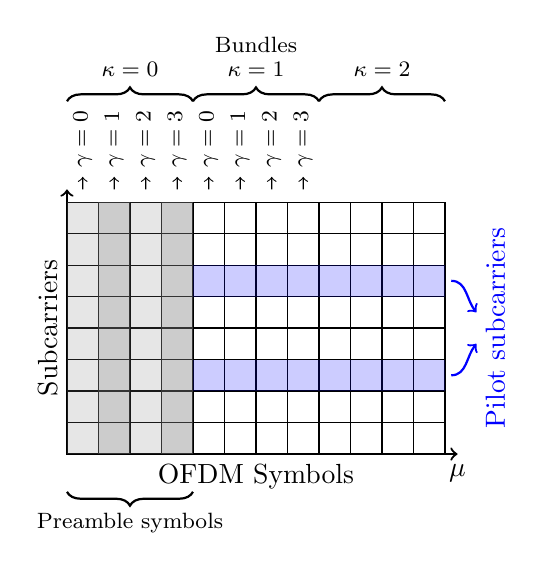
\begin{tikzpicture}[scale=0.8]
% Draw axes
    \draw [<->,thick] (0,4.2) node (yaxis) [left] {}
        |- (6.2,0) node (xaxis) [below] {$\mu$};
%    \node[left] at (0,5-\DELTA/2) {\footnotesize $m=0$};    
%    \node[left, text centered] at (0,\DELTA/2) {\footnotesize $m=N_\text{c}-1$};    
%    \node[below] at (\DELTA/2,0 ) {\footnotesize $\mu = 0$}; 
    \node[left, anchor=south, rotate=90] at (0,2.0) {Subcarriers};
    \node[below] at (3,0) {OFDM Symbols};
% Draw grid
	\draw[step=\DELTA,black,thin,xshift=0cm,yshift=0cm] (0,0) grid (6,4);
%	\draw[step=\DELTA,black,thin, dashed,xshift=0cm,yshift=0cm] (3,0) grid (3.9,4);
% Draw colors
	\draw[draw=none, fill=gray, opacity=0.2] (0,0) rectangle ++(\DELTA, 4);
	\draw[draw=none, fill=gray, opacity=0.4] (\DELTA,0) rectangle ++(\DELTA, 4);
	\draw[draw=none, fill=gray, opacity=0.2] (2*\DELTA,0) rectangle ++(\DELTA, 4);
	\draw[draw=none, fill=gray, opacity=0.4] (3*\DELTA,0) rectangle ++(\DELTA, 4);
%	\draw[draw=none, fill=blue, opacity=0.2] (4*\DELTA,7*\DELTA) rectangle ++(2,\DELTA);


%% channel estimates
%	% nodes
%\node (h0) at (0.25, 5.7) {\footnotesize $\veh{h}_0$};
%\node (h1) at (0.75, 5.4) {\footnotesize $\veh{h}_1$};
%\node (h2) at (1.25, 5.1) {\footnotesize $\veh{h}_2$};
%\node (h3) at (1.75, 4.8) {\footnotesize $\veh{h}_3$};

%% arrows
%  \draw[->, to path={-| (\tikztotarget)}]
%  (0.25,4.2) -- (h0);
%  \draw[->, to path={-| (\tikztotarget)}]
%  (0.75,4.2) -- (h1);
%  \draw[->, to path={-| (\tikztotarget)}]
%  (1.25,4.2) -- (h2);
%  \draw[->, to path={-| (\tikztotarget)}]
%  (1.75,4.2) -- (h3);
  
% Pilots
\draw[draw=none, fill=blue, opacity=0.2] (2,1) rectangle ++(4,\DELTA);
\draw[draw=none, fill=blue, opacity=0.2] (2,2.5) rectangle ++(4,\DELTA);
\draw [->,blue, thick] (6.1, 2.75) to [out=0,in=130] (6.5, 2.25);
\draw [->,blue, thick] (6.1, 1.25) to [out=0,in=-130] (6.5, 1.75);
\node[right, anchor=center, rotate=90, color = blue] at (6.8, 2.0) {Pilot subcarriers};

%% Pilot tone
%	\node (pilot) at (3.25,5.0) {\footnotesize \color{blue}Reference tone\color{black}};
%  \draw[->, to path={-| (\tikztotarget)}, blue]
%  (3.25,3.75) -- (pilot);

% slow-time

% Draw preambles
\draw[decorate,decoration={brace,amplitude=5pt}, thick]  (0,5.6) -- (2,5.6);
\node (pr0) at (1, 6.1) {\footnotesize $\kappa = 0$};
\draw[decorate,decoration={brace,amplitude=5pt}, thick]  (2,5.6) -- (4,5.6);
\node (s0) at (3, 6.1) {\footnotesize $\kappa = 1$};
\draw[decorate,decoration={brace,amplitude=5pt}, thick]  (4,5.6) -- (6,5.6);
\node (s1) at (5, 6.1) {\footnotesize $\kappa = 2$};

\node[align=center] (cu0) at (3, 6.5) {\footnotesize Bundles};


% gamma symbols
\node[right, rotate=90] (g5) at (0.25, 4.4) {\footnotesize $\gamma = 0$};
\node[right, rotate=90] (g6) at (0.75, 4.4) {\footnotesize $\gamma = 1$};
\node[right, rotate=90] (g7) at (1.25, 4.4) {\footnotesize $\gamma = 2$};
\node[right,  rotate=90] (g8) at (1.75, 4.4) {\footnotesize $\gamma = 3$};


\node[right, rotate=90] (g1) at (2.25, 4.4) {\footnotesize $\gamma = 0$};
\node[right, rotate=90] (g2) at (2.75, 4.4) {\footnotesize $\gamma = 1$};
\node[right, rotate=90] (g3) at (3.25, 4.4) {\footnotesize $\gamma = 2$};
\node[right, rotate=90] (g4) at (3.75, 4.4) {\footnotesize $\gamma = 3$};


\draw[->, to path={-| (\tikztotarget)}]
  (2.25,4.2) -- (g1);
  \draw[->, to path={-| (\tikztotarget)}]
  (2.75,4.2) -- (g2);
  \draw[->, to path={-| (\tikztotarget)}]
  (3.25,4.2) -- (g3);
  \draw[->, to path={-| (\tikztotarget)}]
  (3.75,4.2) -- (g4);
  \draw[->, to path={-| (\tikztotarget)}]
  (0.25,4.2) -- (g5);
  \draw[->, to path={-| (\tikztotarget)}]
  (0.75,4.2) -- (g6);
  \draw[->, to path={-| (\tikztotarget)}]
  (1.25,4.2) -- (g7);
  \draw[->, to path={-| (\tikztotarget)}]
  (1.75,4.2) -- (g8);
 
 \node[right, anchor=center, align=center] at (5.0, 5.0) {$\hdots$};
 
 \draw[decorate,decoration={brace,amplitude=5pt}, thick, anchor=center, rotate=180]  (-2,0.6) -- (0,0.6);
 \node[align=center] (cu0) at (1, -1.1) {\footnotesize Preamble symbols};
  
%\node[right, anchor=center, align=center] at (1.0, 0.7) {$\vdots$};
%\node[right, anchor=center, align=center] at (4.0, 0.7) {$\vdots$};

\end{tikzpicture}
\caption{Exemplary allocation of preamble OFDM symbols and pilot subcarriers in $\m{S}$ for DDM.}
\label{fig:Comm_setup_DDM}
\end{figure}





\subsubsection{Synchronization of the Preamble OFDM Symbols} 

The model in \eqref{equ:MODEL_DDM_prea002}  serves as a basis for synchronization, however, as usual in channel estimation, the roles of the channel and the preamble \ac{ofdm} symbols are reversed. This yields
\begin{align}
	\ve{z}_{\kappa, \gamma} &={}  \m{X}_\text{pr}  \ve{h}_{\gamma} \text{e}^{\text{j} \varphi_{\kappa, \gamma}} + \ve{n}_{\kappa, \gamma}, \label{equ:IEEE_DDM_prea001} 
\end{align}
where $\m{X}_\text{pr} = \text{diag}\left( \ve{x}_\text{pr}  \right)\in \mathbb{C}^{N_\text{c} \times N_\text{c}}$.  Without loss of generality, $\varphi_{0,\gamma}$ is set to $0$ and we estimate the \ac{cpe} within $\ve{z}_{\kappa, \gamma}$ with respect to $\ve{z}_{0, \gamma}$ via \cite{classen1994frequency, Diss_Hofbauer, huemer2002simulation }
\begin{align}
\widehat{\varphi}_{\kappa,\gamma} = \text{arg} \left( \ve{z}_{0, \gamma}^H  \ve{z}_{\kappa,\gamma} \right),	 \label{equ:IEEE__DDM_prea_pilot006a} 
\end{align}
whereas $\veh{\cdot}$ indicates that $\widehat{\varphi}_{\kappa,\gamma} $ is an estimate of $\varphi_{\kappa, \gamma} $.  This estimation procedure is repeated for $0 \leq \gamma < 4$ and for $0 \leq \kappa < N_\text{pr}/4$. The estimated \acp{cpe} are then used to synchronize $\ve{z}_{\kappa, \gamma}$ according to
\begin{align}
\vef{z}_{\kappa,\gamma} &={} \ve{z}_{\kappa,\gamma} \cdot \text{e}^{-\text{j} \widehat{\varphi}_{\kappa,\gamma} }.	 \label{equ:IEEE__DDM_prea_pilot007} 
\end{align}
After synchronization, averaging within one bundle yields
\begin{align}
	\bar{\vef{z}}_{\gamma} = \frac{1}{N_\text{pr}/4} \sum_{\kappa=0}^{N_\text{pr}/4-1}  \vef{z}_{\kappa,\gamma}.  \label{equ:IEEE_CIR015ddd}	
\end{align}
With \eqref{equ:DDM_001} and \eqref{equ:IEEE_CIR015ddd}, \eqref{equ:IEEE_DDM_prea001} can be approximated by 
\begin{align}
	\bar{\vef{z}}_{\gamma} &\approx{}  \underbrace{\m{X}_\text{pr} \m{F}_{N_\text{c}} \m{B}_{\text{zp}}}_{\m{M}_\text{pr}} \ve{g}_{\gamma} + \underbrace{\frac{1}{N_\text{pr}/4} \sum_{\kappa=0}^{N_\text{pr}/4-1}  \ve{n}_{\kappa,\gamma}}_{\ve{n}_{ \gamma}} \\
	&={} \m{M}_\text{pr} \ve{g}_{\gamma} + \ve{n}_{ \gamma}, \label{equ:IEEE_CIR0329}
\end{align}
%The incorporation of \eqref{equ:DDM_001} yields
%\begin{align}
%	\bar{\vef{z}}_{\gamma} &={} \underbrace{\m{X}_\text{pr} \m{F}_{N_\text{c}} \m{B}_{\text{zp}}}_{\m{M}_\text{pr}} \ve{g}_{\gamma} + \underbrace{\frac{1}{N_\text{pr}/4} \sum_{\kappa=0}^{N_\text{pr}/4-1}  \ve{n}_{\kappa,\gamma}}_{\ve{n}_{ \gamma}} \\
%	&={} \m{M}_\text{pr} \ve{g}_{\gamma} + \ve{n}_{ \gamma}, \label{equ:IEEE_CIR0329} 
%\end{align}
which is the basis for the following estimation procedure.


\subsubsection{ECIR/ECFR Estimation} 

Employing the commonly used \ac{blue} \cite{Kay-Est.Theory, salehi2007digital, Lang_Asilomar_2014, Diss_Lang_Oliver} on \eqref{equ:IEEE_CIR0329}, an estimate of the \ac{ecir} $\ve{g}_{\gamma}$ follows as
\begin{align}
	\veh{g}_{\gamma} =  \left(\m{M}_\text{pr}^H \m{M}_\text{pr}\right)^{-1} \m{M}_\text{pr}^H \bar{\vef{z}}_{\gamma}.  \label{equ:IEEE_CIR015}	
\end{align}
The estimated \acp{ecir} in \eqref{equ:IEEE_CIR015} can be transformed into an estimate of the corresponding \acp{ecfr} $\ve{h}_{\gamma}$ via 
\begin{align}
\veh{h}_{\gamma} = \m{F}_{N_\text{c}} \m{B}_{\text{zp}} \veh{g}_{\gamma}. \label{equ:DDM_002}
\end{align}
The matrix representation of the estimate $\veh{h}_{\gamma}$ is defined as $\mh{H}_{\gamma} = \text{diag}\left( \veh{h}_{\gamma}  \right)\in \mathbb{C}^{N_\text{c} \times N_\text{c}}$. This procedure is repeated for all indexes $\gamma = 0, \hdots, 3$. 


\subsection{Synchronization of OFDM Symbols for $\kappa \geq N_\text{pr}/4$} 

Considering only the pilot subcarriers of the model in \eqref{equ:MODEL_DDM_prea001} and replacing the \ac{ecfr} by its estimate yields
\begin{align}
	\ve{z}_{\kappa, \gamma}^\text{p} &\approx{} \mh{H}_{\gamma}^\text{p}  \underbrace{\ve{s}_{\kappa, \gamma}^\text{p} \text{e}^{\text{j} \varphi_{\kappa, \gamma}}}_{\ve{t}_{\kappa, \gamma}^\text{p}} + \ve{n}_{\kappa, \gamma}^\text{p} \\
	&={} \mh{H}_{\gamma}^\text{p} \ve{t}_{\kappa, \gamma}^\text{p} + \ve{n}_{\kappa, \gamma}^\text{p}, \label{equ:IEEE_pilot000} 
\end{align}
where $\ve{t}_{\kappa, \gamma}^\text{p} = \ve{s}_{\kappa, \gamma}^\text{p} \text{e}^{\text{j} \varphi_{\kappa, \gamma}} \in \mathbb{C}^{N_\text{p}}$ represents \ac{cpe} distorted pilot symbols  \cite{Hofbauer20_2, Hofbauer20_2a}. Employing the commonly used \ac{lmmse} estimator \cite{Kay-Est.Theory, Diss_Hofbauer,  huemer2011classical, huemer2002simulation, classen1994frequency, Diss_Lang_Oliver, Lang_RDM_JP} on \eqref{equ:IEEE_pilot000} yields
\begin{align}
\veh{t}_{\kappa, \gamma}^\text{p} &={}  \left( \left(\mh{H}_{\gamma}^\text{p} \right)^H \mh{H}_{\gamma}^\text{p} + N_\text{c} \sigma_\text{n}^2 \m{C}_{\ve{t}\ve{t}}^{-1} \right)^{-1}  \left(\mh{H}_{\gamma}^\text{p} \right)^H \ve{z}_{\kappa, \gamma}^\text{p}.	 \label{equ:IEEE_pilot005a} 
\end{align}
There, $\m{C}_{\ve{t}\ve{t}}\in \mathbb{C}^{N_\text{p} \times N_\text{p}}$ denotes the covariance matrix of $\ve{t}_{\kappa, \gamma}^\text{p}$ and it is assumed to be a diagonal matrix for simplicity. The diagonal elements of $\m{C}_{\ve{t}\ve{t}}$ represent the pilot symbols' average power (averaged over the \ac{ofdm} symbols). The estimate \ac{cpe} distorted pilot symbols $\veh{t}_{\kappa, \gamma}^\text{p}$ in \eqref{equ:IEEE_pilot005a} 
feature the error covariance matrix  \cite{Diss_Hofbauer, Kay-Est.Theory, Diss_Lang_Oliver}
\begin{align}
\m{C}_{ee}^\text{p} &={} N_\text{c} \sigma_\text{n}^2 \left( \left(\mh{H}_{\gamma}^\text{p} \right)^H \mh{H}_{\gamma}^\text{p} + N_\text{c} \sigma_\text{n}^2 \m{C}_{\ve{t}\ve{t}}^{-1} \right)^{-1} .	 \label{equ:IEEE_pilot006} 
\end{align}
Comparing the estimates $\veh{t}_{\kappa, \gamma}^\text{p}$ in \eqref{equ:IEEE_pilot005a} with the known transmitted pilot symbols $\ve{s}_{\kappa, \gamma}^\text{p}$ allows estimating the \ac{cpe} for every $\kappa \geq N_\text{pr}/4$ and for $ 0 \leq \gamma < 4$ according to \cite{classen1994frequency, Diss_Hofbauer, huemer2002simulation}
\begin{align}
\widehat{\varphi}_{\kappa, \gamma} = \text{arg} \left( \left( \ve{s}_{\kappa, \gamma}^\text{p} \right)^H\m{W}\, \veh{t}_{\kappa, \gamma}^\text{p} \right).	 \label{equ:IEEE_pilot006a} 
\end{align}
Here, the diagonal matrix $\m{W}\in \mathbb{C}^{N_\text{p} \times N_\text{p}}$ weights the estimated pilot subcarriers based on their estimation accuracy indicated by $\m{C}_{ee}^\text{p}$ in \eqref{equ:IEEE_pilot006} \cite{Diss_Hofbauer, Lang_RDM_JP}. 
Finally, the estimated \acp{cpe} are used for de-rotating the received data subcarriers according to
\begin{align}
\vef{z}_{\kappa, \gamma}^\text{d} &={}  \ve{z}_{\kappa, \gamma}^\text{d} \cdot \text{e}^{-\text{j} \widehat{\varphi}_{\kappa, \gamma} }.	 \label{equ:IEEE_pilot007} 
\end{align}





\subsection{Data Estimation} 

Recall that the same data symbols are transmitted over 4 consecutive \ac{ofdm} symbols according to \eqref{equ:Comm_OFDM_00111}. Hence, the 4 vectors $\vef{z}_{\kappa, 0}^\text{d}, \cdots, \vef{z}_{\kappa, 3}^\text{d}$ are used to estimate the data symbols in $\ve{x}_{\kappa}^\text{d} $. The connection between these vectors is given by
\begin{align}
	\underbrace{\begin{bmatrix}
	\vef{z}_{\kappa, 0}^\text{d} \\
	\vef{z}_{\kappa, 1}^\text{d} \\
	\vef{z}_{\kappa, 2}^\text{d} \\
	\vef{z}_{\kappa, 3}^\text{d}  
	\end{bmatrix}}_{\vef{z}_{\kappa}^\text{d}\in \mathbb{C}^{4N_\text{d}}}
	&={}  \underbrace{\begin{bmatrix}  
\mh{H}_{0}^\text{d}  \\
\mh{H}_{1}^\text{d}  \\ 
\mh{H}_{2}^\text{d}  \\  
\mh{H}_{3}^\text{d}  \end{bmatrix}}_{\mh{H}^\text{d}\in \mathbb{C}^{4N_\text{d}\times N_\text{d}}} 
\ve{x}_{\kappa}^\text{d} + \underbrace{\begin{bmatrix}
	\ve{n}_{\kappa,0}^\text{d} \\
	\ve{n}_{\kappa,1}^\text{d} \\
	\ve{n}_{\kappa,2}^\text{d} \\
	\ve{n}_{\kappa,3}^\text{d} 
	\end{bmatrix}}_{\ve{n}_{\kappa}^\text{d}\in \mathbb{C}^{4N_\text{d}}}   \label{equ:IEEE_CIR032d}  \\ \nonumber \\
\vef{z}_{\kappa}^\text{d} &={} \mh{H}^\text{d} \ve{x}_{\kappa}^\text{d} + \ve{n}_{\kappa}^\text{d}.	 \label{equ:IEEE_CIR032c} 
\end{align}
The \ac{lmmse} estimator for $\ve{x}_{\kappa}^\text{d}$ can be derived as \cite{Diss_Hofbauer, Kay-Est.Theory,  huemer2011classical} 
\begin{align}
\widehat{\ve{x}}_{\kappa}^\text{d} &={}  \left( \left(\mh{H}^\text{d} \right)^H \mh{H}^\text{d} + \frac{N_\text{c} \sigma_\text{n}^2}{\sigma_\text{d}^2} \m{I}^{N_\text{d}} \right)^{-1}  \left(\mh{H}^\text{d} \right)^H \vef{z}_{\kappa}^\text{d},	 \label{equ:IEEE_CIR032e} 
\end{align}
%where $\sigma_\text{d}^2$ denotes the variance of the assumed uncorrelated data symbols. These data symbols are usually normalized such that $\sigma_\text{d}^2=1$.
 representing the final estimate of the data symbols. 


%The corresponding error covariance matrix is given by \cite{Diss_Hofbauer, Kay-Est.Theory}
%\begin{align}
%\m{C}_{ee}^\text{d} &={} N_\text{c} \sigma_\text{n}^2 \left( \left(\mh{H}^\text{d} \right)^H \mh{H}^\text{d} + \frac{N_\text{c} \sigma_\text{n}^2}{\sigma_\text{d}^2} \m{I}^{N_\text{d}} \right)^{-1} .	 \label{equ:IEEE_pilot006C} 
%\end{align}
%Finally, the estimates in \eqref{equ:IEEE_CIR032e} are fed into the de-matter, the de-interleaver and the decoder detailed in the following.







